% Options for packages loaded elsewhere
\PassOptionsToPackage{unicode}{hyperref}
\PassOptionsToPackage{hyphens}{url}
%
\documentclass[
]{article}
\usepackage{lmodern}
\usepackage{amssymb,amsmath}
\usepackage{ifxetex,ifluatex}
\ifnum 0\ifxetex 1\fi\ifluatex 1\fi=0 % if pdftex
  \usepackage[T1]{fontenc}
  \usepackage[utf8]{inputenc}
  \usepackage{textcomp} % provide euro and other symbols
\else % if luatex or xetex
  \usepackage{unicode-math}
  \defaultfontfeatures{Scale=MatchLowercase}
  \defaultfontfeatures[\rmfamily]{Ligatures=TeX,Scale=1}
\fi
% Use upquote if available, for straight quotes in verbatim environments
\IfFileExists{upquote.sty}{\usepackage{upquote}}{}
\IfFileExists{microtype.sty}{% use microtype if available
  \usepackage[]{microtype}
  \UseMicrotypeSet[protrusion]{basicmath} % disable protrusion for tt fonts
}{}
\makeatletter
\@ifundefined{KOMAClassName}{% if non-KOMA class
  \IfFileExists{parskip.sty}{%
    \usepackage{parskip}
  }{% else
    \setlength{\parindent}{0pt}
    \setlength{\parskip}{6pt plus 2pt minus 1pt}}
}{% if KOMA class
  \KOMAoptions{parskip=half}}
\makeatother
\usepackage{xcolor}
\IfFileExists{xurl.sty}{\usepackage{xurl}}{} % add URL line breaks if available
\IfFileExists{bookmark.sty}{\usepackage{bookmark}}{\usepackage{hyperref}}
\hypersetup{
  pdftitle={Instance Space Analysis on Quantum Algorithms},
  pdfauthor={Vivek Katial},
  hidelinks,
  pdfcreator={LaTeX via pandoc}}
\urlstyle{same} % disable monospaced font for URLs
\usepackage[margin=1in]{geometry}
\usepackage{graphicx,grffile}
\makeatletter
\def\maxwidth{\ifdim\Gin@nat@width>\linewidth\linewidth\else\Gin@nat@width\fi}
\def\maxheight{\ifdim\Gin@nat@height>\textheight\textheight\else\Gin@nat@height\fi}
\makeatother
% Scale images if necessary, so that they will not overflow the page
% margins by default, and it is still possible to overwrite the defaults
% using explicit options in \includegraphics[width, height, ...]{}
\setkeys{Gin}{width=\maxwidth,height=\maxheight,keepaspectratio}
% Set default figure placement to htbp
\makeatletter
\def\fps@figure{htbp}
\makeatother
\setlength{\emergencystretch}{3em} % prevent overfull lines
\providecommand{\tightlist}{%
  \setlength{\itemsep}{0pt}\setlength{\parskip}{0pt}}
\setcounter{secnumdepth}{-\maxdimen} % remove section numbering
\widowpenalties 1 150
\usepackage{amssymb}
\usepackage{amsmath}
\usepackage{amsthm}
\usepackage{braket}
\usepackage{xcolor}
\usepackage[ruled,vlined]{algorithm2e}
\SetAlFnt{\small}
\SetAlCapFnt{\large}
\SetAlCapNameFnt{\large}
\usepackage{algorithmic}
\algsetup{linenosize=\tiny}

\title{Instance Space Analysis on Quantum Algorithms}
\author{Vivek Katial}
\date{20/07/2020}

\begin{document}
\maketitle

\hypertarget{introduction}{%
\section{Introduction}\label{introduction}}

\hypertarget{about-me}{%
\subsection{About Me}\label{about-me}}

\begin{itemize}
\tightlist
\item
  Vivek Katial
  (\href{mailto:vkatial@student.unimelb.edu.au}{\nolinkurl{vkatial@student.unimelb.edu.au}})

  \begin{itemize}
  \tightlist
  \item
    PhD Candidate in School of Mathematics and Statistics
  \end{itemize}
\end{itemize}

\hypertarget{talk-structure}{%
\subsection{Talk Structure}\label{talk-structure}}

\begin{itemize}
\tightlist
\item
  Background
\item
  Overview of Literature
\item
  Current Progress
\item
  What's next?
\end{itemize}

\hypertarget{main-research-question}{%
\subsection{Main Research Question}\label{main-research-question}}

\begin{itemize}
\tightlist
\item
  What instances characteristics of optimisation problems make them
  predisposed to being solved on a Quantum Computer?
\end{itemize}

\hypertarget{adiabatic-quantum-computing-aqc}{%
\section{Adiabatic Quantum Computing
(AQC)}\label{adiabatic-quantum-computing-aqc}}

\hypertarget{adiabatic-quantum-computing-aqc-1}{%
\subsection{Adiabatic Quantum Computing
(AQC)}\label{adiabatic-quantum-computing-aqc-1}}

\begin{quote}
\begin{itemize}
\tightlist
\item
  Adiabatic Quantum Computation is a computational model which relies on
  the \emph{adiabatic thereom} of quantum mechanics to compute
  calculations.
\item
  The famous \emph{Schrödinger Equation} is well-known to describe the
  time evolution of a quantum state:
\end{itemize}
\end{quote}

\begin{quote}
\begin{itemize}
\tightlist
\item
  \[
  i\hbar \frac{d}{dt} \ket{\psi (t)} = H(t) \ket{\psi(t)}
  \]
\end{itemize}
\end{quote}

\begin{quote}
\begin{itemize}
\tightlist
\item
  \(\ket{\psi(t)}\) is our state vector, \(H(t)\) is the time dependent
  Hamiltonian. A Hamiltonian of an \(n\)-qubit system \(H(t)\) is given
  by \(2^n \times 2^n\) matrix.
\end{itemize}
\end{quote}

\hypertarget{adiabatic-quantum-computing-aqc-2}{%
\subsection{Adiabatic Quantum Computing
(AQC)}\label{adiabatic-quantum-computing-aqc-2}}

\begin{quote}
\begin{itemize}
\tightlist
\item
  An adiabatic computation can be expressed by specifying two
  Hamiltonians, denoted by \(H_B\) and \(H_P\) where \(H_B\) is our
  \emph{initial} Hamiltonian and \(H_P\) is the \emph{final} or
  \emph{problem} Hamiltonian.
\item
  \[\begin{matrix}
  H_B &  \xrightarrow{\hspace*{3cm}} & H_P \\
  \ket{\psi_B} &  \text{transform } H(t) &  \ket{\psi_P} \\
  \text{known state} &  &  \text{unknown}
  \end{matrix}
  \]
\item
  Loosely speaking, the adiabatic theorem tells us that if we vary from
  \(H_B\) to \(H_P\) \emph{slowly enough} the system will remain in its
  ground state. This fact is a direct result of the Adiabatic Theorem
  {[}1{]}.
\end{itemize}
\end{quote}

\hypertarget{adiabatic-quantum-computing-aqc-3}{%
\subsection{Adiabatic Quantum Computing
(AQC)}\label{adiabatic-quantum-computing-aqc-3}}

\begin{quote}
\begin{itemize}
\tightlist
\item
  To conduct the computation we evolve \(\ket{\psi(t)}\) till time
  \(t=T\) such that \(\ket{\psi(t=T)}\) encodes the answer. The
  computation is done using a Hamiltonian which interpolates between
  \(H_B\) and \(H_P\). Specifically as below:
\end{itemize}
\end{quote}

\begin{quote}
\begin{itemize}
\tightlist
\item
  \[
  H(t) = \left[1 - \lambda(t)\right]H_B + \lambda(t)H_P, \qquad \lambda (t) = \frac{t}{T}
  \]
\item
  How fast?
\item
  \[
  T =  \frac{1}{\min_t  g(t)^2}
  \]
\item
  Where \(g(t)\) is the difference between the first two smallest
  eigenvalues of \(H(t)\)
\end{itemize}
\end{quote}

\hypertarget{sat---exact-cover}{%
\section{3SAT - Exact Cover}\label{sat---exact-cover}}

\hypertarget{sat-exact-cover}{%
\subsection{3SAT (Exact Cover)}\label{sat-exact-cover}}

\begin{quote}
\begin{itemize}
\tightlist
\item
  The satisfiability problem, abbreviated SAT, is a classic example of
  an NP-complete problem {[}2{]}
\item
  The basic SAT formulation can be described as follows: Given a boolean
  formula (AND \(\land\), OR \(\lor\) , NOT \(\neg\)) over \(n\)
  variables (\(z_1, z_2, ... , z_n\)). Can one set \(z_i\)'s in a manner
  such that the Boolean formula is true?
\item
  A clause is an expression which the variables must satisfy. For
  example \(z_1 \land z_2 \implies z_1 = z_2 = 1\)
\end{itemize}
\end{quote}

\hypertarget{sat-exact-cover-example}{%
\subsection{3SAT (Exact Cover Example)}\label{sat-exact-cover-example}}

\begin{quote}
\begin{itemize}
\tightlist
\item
  Consider a 4-bit number with two clauses:

  \begin{itemize}
  \tightlist
  \item
    \(z_1 \land z_2 \land z_3\)
  \item
    \(z_1 \land z_3 \land z_4\)
  \end{itemize}
\item
  Here we have 16 possible assignments, namely:
\item
  \begin{align*}
  \mathcal{Z} = \{\,
  & 0000, 0001, 0010, 0011, 0100, 0101, 0110, 0111, \\
  & 1000, 1001, 1010, 1011, 1100, 1101, 1110, 1111 \,\}\enspace
  \end{align*}
\end{itemize}
\end{quote}

\begin{quote}
\begin{itemize}
\tightlist
\item
  However, our \textbf{satisfying assignment} is only \(\vec{z} = 1111\)
\item
  We call a 3SAT problem with one satisfying assignment an instance of
  USA
\item
  Exact Cover implies that clauses are ``exclusive'' and in the form of
  \(z_i + z_j + z_k = 1\)
\end{itemize}
\end{quote}

\hypertarget{mapping-3sat-to-aqc}{%
\subsection{Mapping 3SAT to AQC}\label{mapping-3sat-to-aqc}}

\begin{quote}
\begin{itemize}
\tightlist
\item
  How do we construct \(H_B\) and \(H_P\) so that we can solve our
  optimisation problem?
\item
  Farhi et al.{[}3{]} describe this construction in considerable detail.
\item
  We then evolve our system with the following interpolation:
\item
  \[
  H(t) = \left[1 - \lambda(t)\right]H_B + \lambda(t)H_P, \qquad \lambda (t) = \frac{t}{T}
  \]
\item
  Finally, complete measurement and our solution is our final state
  \(\ket{\psi(t=T)}\)
\end{itemize}
\end{quote}

\hypertarget{instance-space-analysis}{%
\section{Instance Space Analysis}\label{instance-space-analysis}}

\hypertarget{algorithm-selection}{%
\subsection{Algorithm Selection}\label{algorithm-selection}}

\begin{quote}
\begin{itemize}
\tightlist
\item
  Given a set of problem instances, predicting which algorithm is most
  likely to best perform was first explored by Rice {[}4{]}. \pause
\end{itemize}
\end{quote}

\begin{center}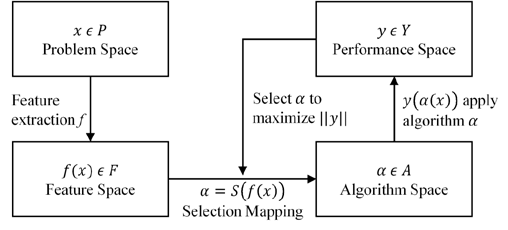
\includegraphics[width=0.6\linewidth]{./rices-framework-for-algorithm-selection} \end{center}

\begin{quote}
\begin{itemize}
\tightlist
\item
  However, what we are interested in is probing the strengths and
  weaknesses of AQC for different instances of SAT.
\end{itemize}
\end{quote}

\hypertarget{instance-space-methodology}{%
\subsection{Instance Space
Methodology}\label{instance-space-methodology}}

\begin{quote}
\begin{itemize}
\tightlist
\item
  The instance space methodology presented in {[}5--7{]} extends Rice's
  framework. \pause
\end{itemize}
\end{quote}

\begin{center}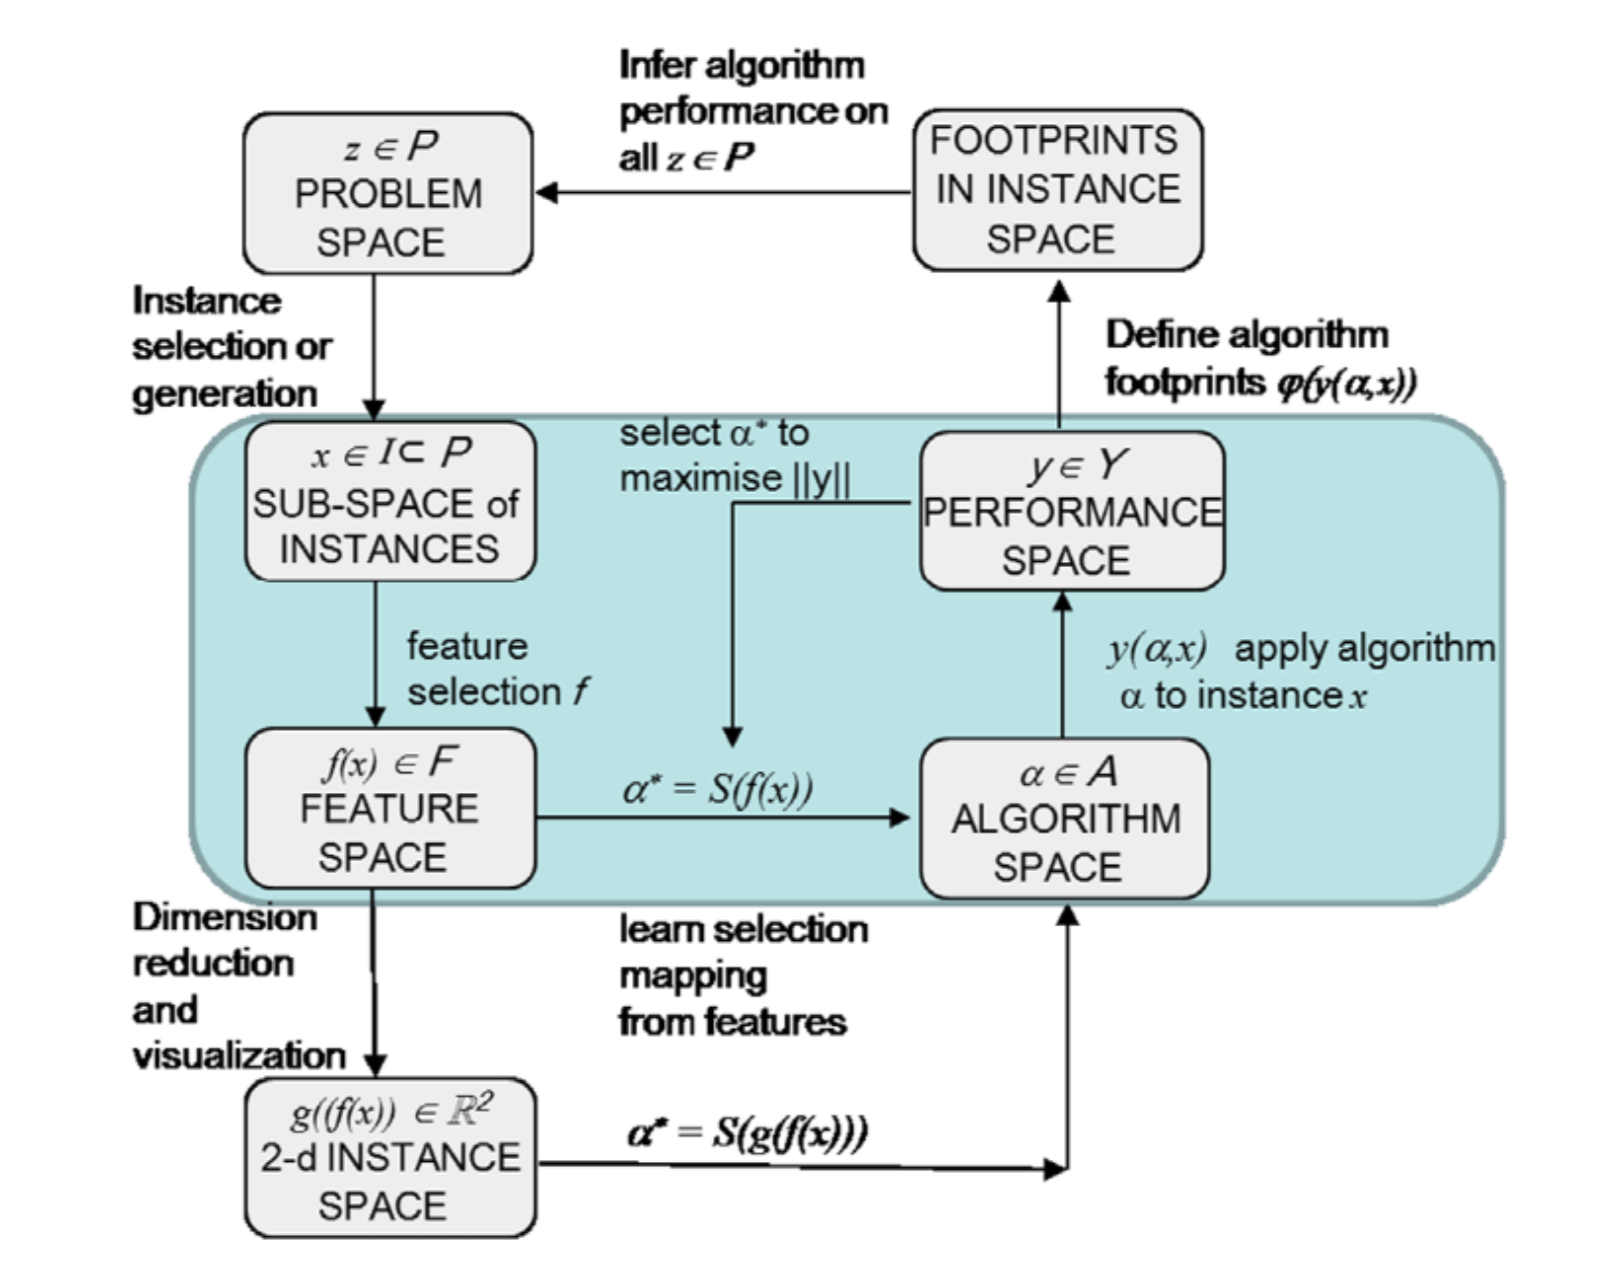
\includegraphics[width=0.6\linewidth]{./instance-space-methodology} \end{center}

\hypertarget{current-literature}{%
\section{Current Literature}\label{current-literature}}

\hypertarget{quantum-computing-research-into-hard-sat-problems}{%
\subsection{Quantum Computing Research into Hard SAT
problems}\label{quantum-computing-research-into-hard-sat-problems}}

\begin{quote}
\begin{itemize}
\tightlist
\item
  In their seminal paper {[}3{]} Farhi et al.~aswell as Hogg et
  al.~{[}8{]} touched on the phase transition and showed that the
  minimum energy gap perhaps scaled polynomially with \(n\) as roughly
  \(N^2\).
\item
  However in 2009, Young et al {[}9{]}. demonstrated via Quantum
  monte-carlo simulations of \(N=256\) that some USA instances have a
  \emph{quantum phase transition}.
\item
  Their research indicated that as \(N \rightarrow \infty\) the system
  is expected to lead to an exponentially small gap, and hence an
  exponential complexity.
\item
  Farhi et al.~{[}10{]} also investigated different evolution paths and
  their results suggested it is possible to overcome the exponentially
  small minimum gap by selecting random initial Hamiltonians
\end{itemize}
\end{quote}

\hypertarget{quantum-computing-research-into-hard-sat-problems-1}{%
\subsection{Quantum Computing Research into Hard SAT
problems}\label{quantum-computing-research-into-hard-sat-problems-1}}

\begin{quote}
\begin{itemize}
\tightlist
\item
  Latorre et al.~probed the entropy of entanglement for 250 USA
  Instances of Exact-Cover {[}11{]}, their results showed that entropy
  of entanglement scales linearly with \(N\).
\item
  However, their results also showed that for large \(N\), the minimum
  gap scaling is exponential and can be associated with a \emph{quantum
  phase transition} {[}11{]}.
\item
  Hauke et al.~{[}12{]} ran simulations of adiabatic quantum
  optimisation with \(n=16\). Their results indicated that large
  entanglement entropy has little significance for the success
  probability of the optimisation task.
\end{itemize}
\end{quote}

\hypertarget{quantum-computing-research-into-hard-sat-problems-d-wave}{%
\subsection{Quantum Computing Research into Hard SAT problems
(D-Wave)}\label{quantum-computing-research-into-hard-sat-problems-d-wave}}

\begin{quote}
\begin{itemize}
\tightlist
\item
  Mapping optimisation problems as QUBO problems unlocks a significant
  number of NP-complete problems to investigate {[}13{]}
\item
  Katzgrabber et al.~{[}14{]} found Quantum annealing performed slightly
  better than classical ML algorithms on a computational biology problem
\item
  Gabor et al.~{[}15{]} shows that the phase transition from 3SAT
  persists in some form (but possibly to a lesser extent) in AQC via
  \textbf{real experimental results} on D-WAVE.
\item
  Other promising studies in election forecasting and human cancer
  detection {[}16{]}.
\item
  Current approaches fail to investigate a suitable class of instances.
\end{itemize}
\end{quote}

\hypertarget{research-overview}{%
\section{Research Overview}\label{research-overview}}

\hypertarget{research-overview-1}{%
\subsection{Research Overview}\label{research-overview-1}}

\begin{quote}
\begin{itemize}
\tightlist
\item
  Depending on different structures of instances, classical algorithms
  may perform differently to Quantum ones.
\item
  We are looking to investigate which types of instances are more
  pre-disposed to being solved on Quantum Computers. Currently, we have
  explored two types of instances:

  \begin{itemize}
  \tightlist
  \item
    Relaxed USA Instances
  \item
    Generalised USA Instances
  \end{itemize}
\end{itemize}
\end{quote}

\hypertarget{research-overview-2}{%
\subsection{Research Overview}\label{research-overview-2}}

\begin{quote}
\begin{itemize}
\tightlist
\item
  We then have simulated AQC and probe the ``quantumness'' of each
  instance by measuring:

  \begin{enumerate}
  \def\labelenumi{\arabic{enumi}.}
  \tightlist
  \item
    Minimum Energy Gap \(g_{\text{min}}\)
  \item
    Bipartite Entropy of Entanglement
  \item
    Probability of sucess after a fixed run time \(T\)
  \end{enumerate}
\end{itemize}
\end{quote}

\hypertarget{research-overview---instance-space}{%
\subsection{Research Overview - Instance
Space}\label{research-overview---instance-space}}

\begin{quote}
\begin{itemize}
\tightlist
\item
  The problem space \(\mathcal{P}\) consists of all possible 3SAT
  instances of Exact Cover.
\item
  The instance space \(\mathcal{I} \subset \mathcal{P}\) compromises of
  5760 RUSA and GUSA instances. These range from 5 to 11 qubits and are
  randomly generated.
\item
  The feature space \(\mathcal{F}\) consists of 23 different instance
  features generated
\item
  The algorithm portfolio \(\mathcal{A}\) includes 16 algorithm
  parameter configurations for the run time \(T\) and also the time step
  \(\Delta t\). We also are using a single path function \(\lambda(t)\)
\item
  The performance metric \(y \in \mathcal{Y}\) is the probability of
  success for the algorithm.
\end{itemize}
\end{quote}

\hypertarget{research-overview---generating-gusa-instances}{%
\subsection{Research Overview - Generating GUSA
Instances}\label{research-overview---generating-gusa-instances}}

\begin{algorithm}[H]
\SetAlgoLined
 Fix number of bits to $n$\;
 $C=\{\}$\;
 $i=0$\;
 \While{While number of satisfying assignments $> 0$}{
  $C_i$ = Three distinct bits randomly from a uniform distribution\;
  $i = i + 1$\;
  \uIf{number of satisfying assignments $= 1$ }{
  \textbf{return} $(n, \mathbf{C})$\;
  } \uElseIf{number of satisfying assignments = 0}{
    \textbf{restart}\;
    }
    \uElseIf{number of satisfying assignments has decreased}{
    Add $C_i$ into $\mathbf{C}$ \;
  }
 }
 \KwResult{$(n, \mathbf{C})$: $n$ variables with a set of clauses $\mathbf{C}$ }
 \caption{Generalised USA Instances}
 \label{alg:gusa}
\end{algorithm}

\hypertarget{research-overview---generating-rusa-instances}{%
\subsection{Research Overview - Generating RUSA
Instances}\label{research-overview---generating-rusa-instances}}

\begin{algorithm}[H]
\SetAlgoLined
 Fix number of bits to $n$\;
 $C=\{\}$\;
 $i=0$\;
 \While{While number of satisfying assignments $> 0$}{
  $C_i$ = Three distinct bits randomly from a uniform distribution\;
  $i = i + 1$\;
  \uIf{number of satisfying assignments $= 1$ }{
  \textbf{return} $(n, \mathbf{C})$\;
  } \uElseIf{number of satisfying assignments = 0}{
    \textbf{restart}\;
    }
    \Else{
    Add $C_i$ into $\mathbf{C}$ \;
  }
 }
 \KwResult{$(n, \mathbf{C})$: $n$ variables with a set of clauses $\mathbf{C}$ }
 \caption{Relaxed USA Instances}
 \label{alg:rusa}
\end{algorithm}

\hypertarget{research-overview---fx-instance-characterstics}{%
\subsection{\texorpdfstring{Research Overview - \(f(x)\) Instance
Characterstics}{Research Overview - f(x) Instance Characterstics}}\label{research-overview---fx-instance-characterstics}}

\begin{table}[h!]
\scalebox{0.8}{\begin{tabular}{ll}
\hline
\textbf{Feature Group} & \textbf{Feature}                                                                     \\ \hline
Problem Size           & Number of variables: $n$                                                             \\
                       & Number of clauses: $m$                                                               \\
                       & Clause-to-Variable Ratio: $\frac{n}{m}$, $\frac{n}{m}^{2}$,$\frac{n}{m}^{3}$         \\
                       & Inverse Clause-to-Variable Ratio: $\frac{m}{n}$, $\frac{m}{n}^{2}$,$\frac{m}{n}^{3}$ \\
                       & Linearised Clause to Variable Ratio: $|4.26 - \frac{n}{m}|, |4.26 - \frac{n}{m}|^2$, \\
                       & $|4.26 - \frac{n}{m}|^3$                                                             \\
                       &                                                                                      \\ \hline
Variable Clause Graph  & Variable Node Degree:  mean, median, min, max                                        \\
                       & Clause Node Degree :  mean, median, min, max                                         \\
                       &                                                                                      \\ \hline
Variable Graph  &  Node Degree :  mean, median, min, max                                                      \\
                       &                                                                                      \\ \hline
\end{tabular}}
\caption{Instance Features for 3SAT Exact Cover}
\label{table:instance-features}
\end{table}

\hypertarget{research-overview---distribution-of-features}{%
\subsection{Research Overview - Distribution of
Features}\label{research-overview---distribution-of-features}}

\begin{center}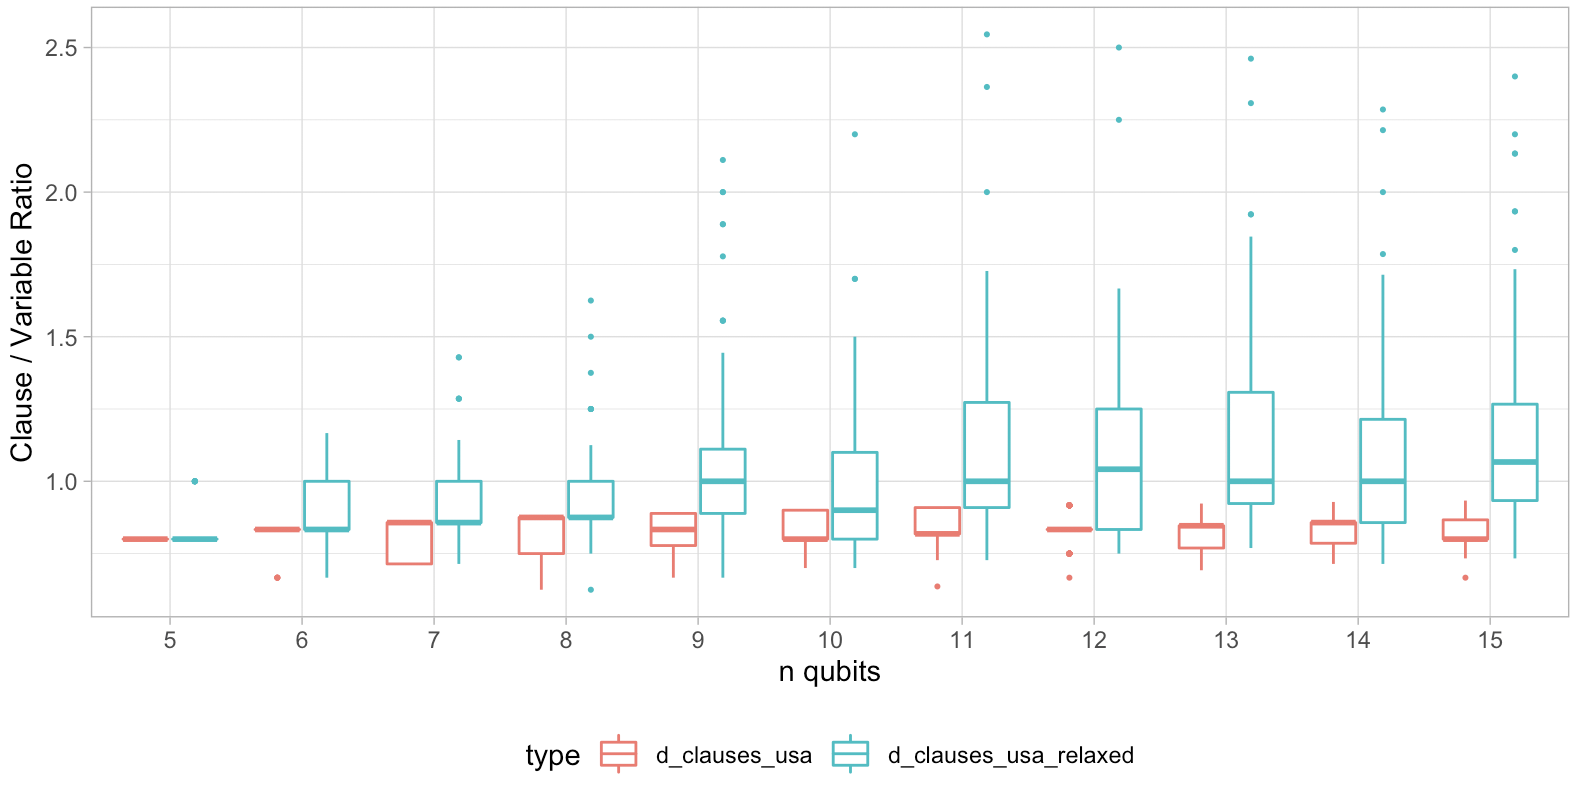
\includegraphics[width=1\linewidth]{./boxplot-instances} \end{center}

\hypertarget{research-overview---distribution-of-features-1}{%
\subsection{Research Overview - Distribution of
Features}\label{research-overview---distribution-of-features-1}}

\begin{center}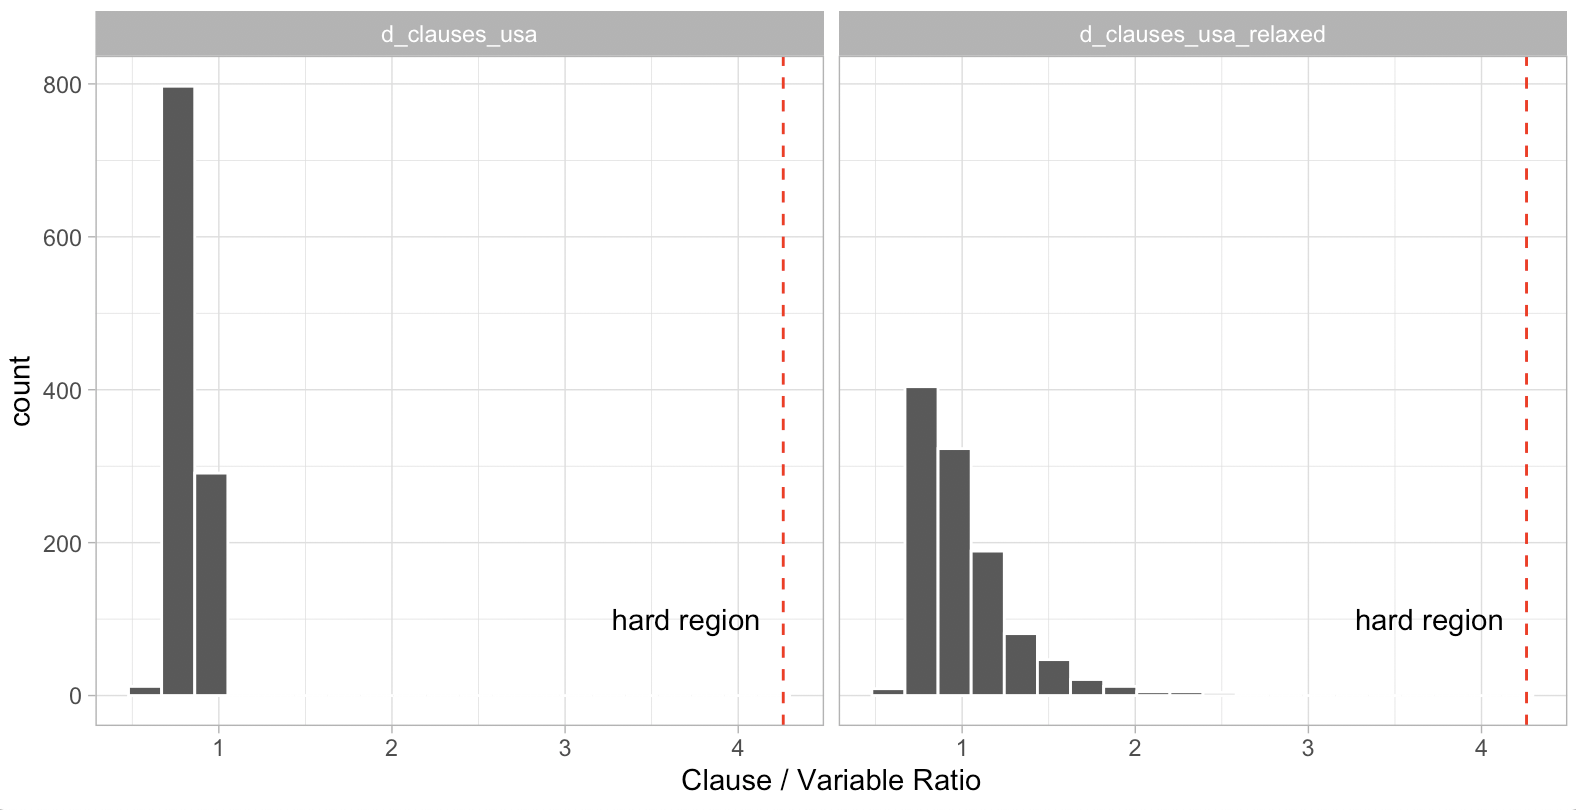
\includegraphics[width=1\linewidth]{./instance-distributions} \end{center}

\hypertarget{results}{%
\section{Results}\label{results}}

\hypertarget{research-overview---results}{%
\subsection{Research Overview -
Results}\label{research-overview---results}}

\begin{center}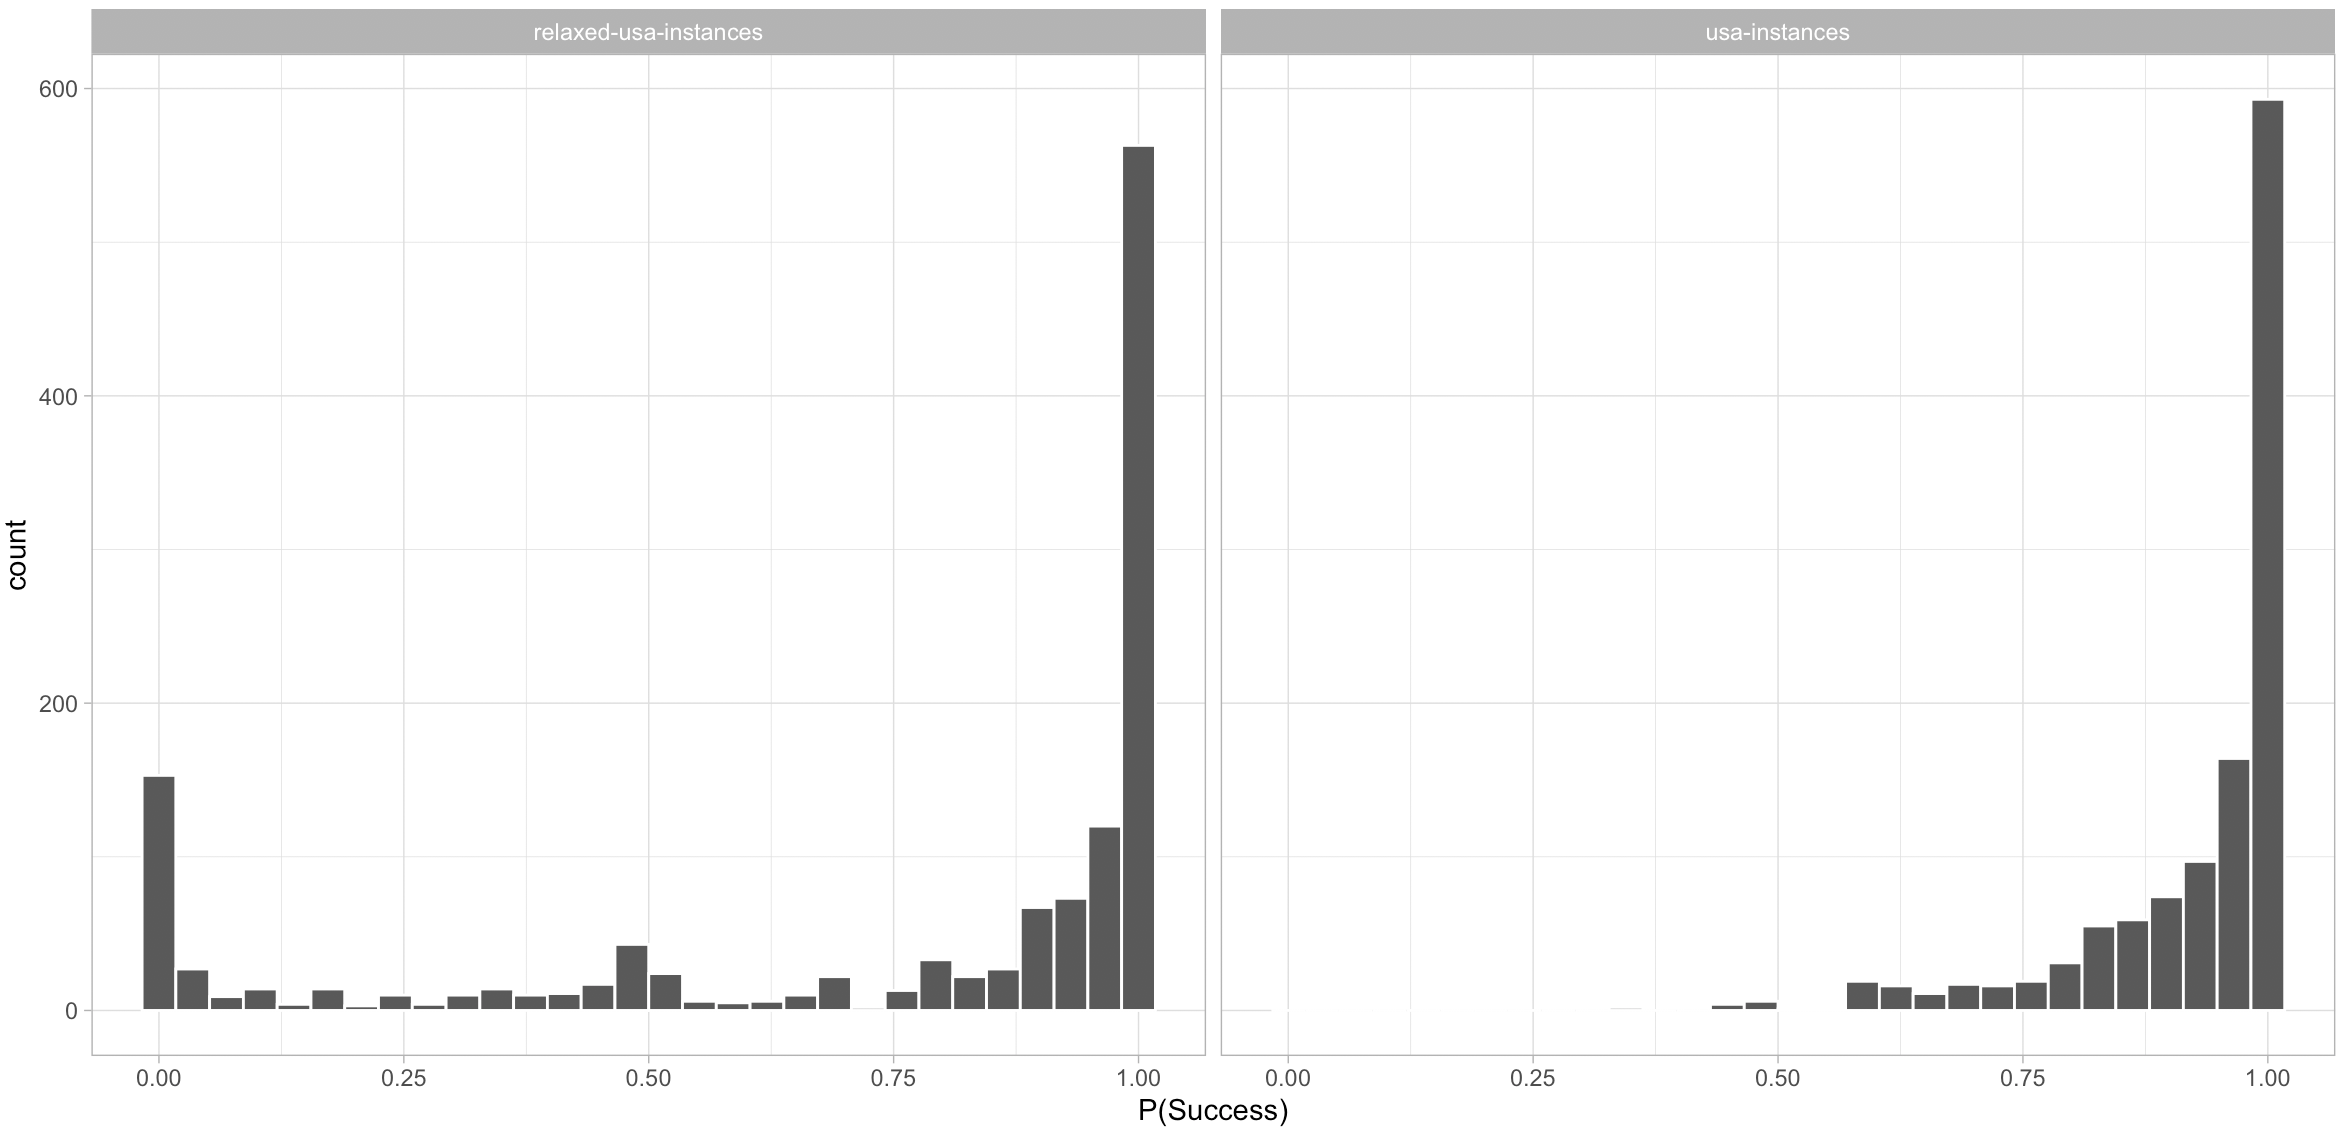
\includegraphics[width=1\linewidth]{./psuccess-instance} \end{center}

\hypertarget{research-overview---results-1}{%
\subsection{Research Overview -
Results}\label{research-overview---results-1}}

\begin{center}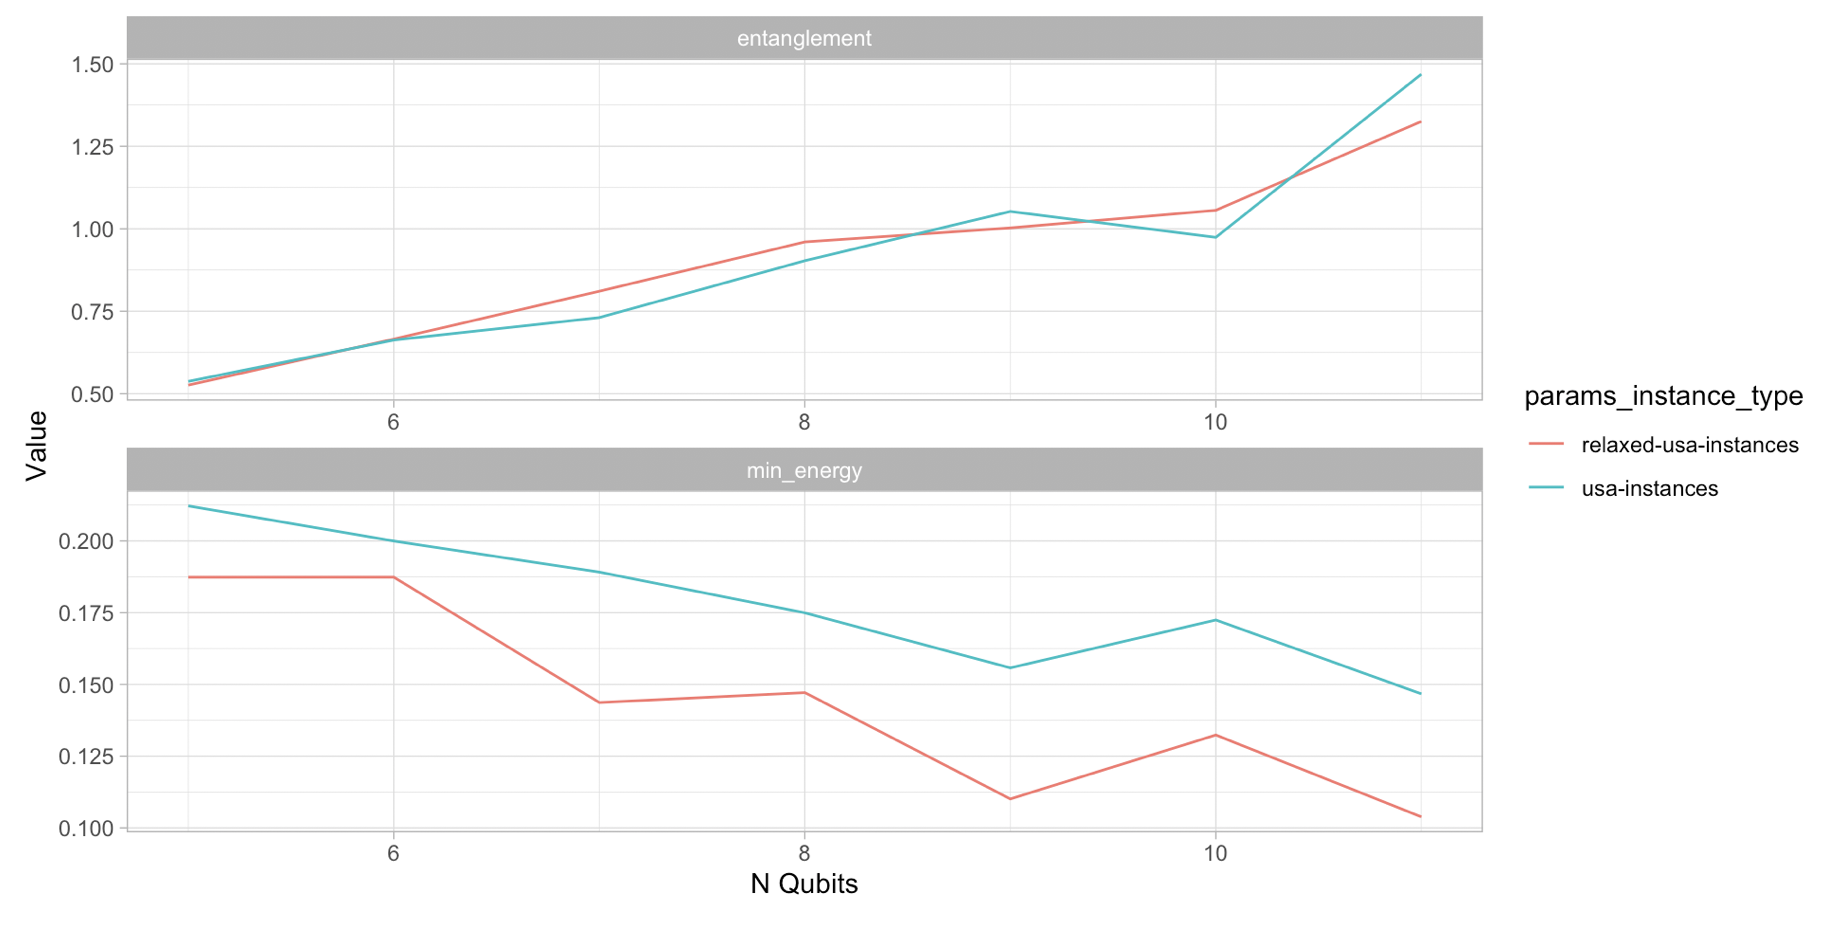
\includegraphics[width=1\linewidth]{./overall-results-by-qubit} \end{center}

\hypertarget{research-overview---results-2}{%
\subsection{Research Overview -
Results}\label{research-overview---results-2}}

\begin{center}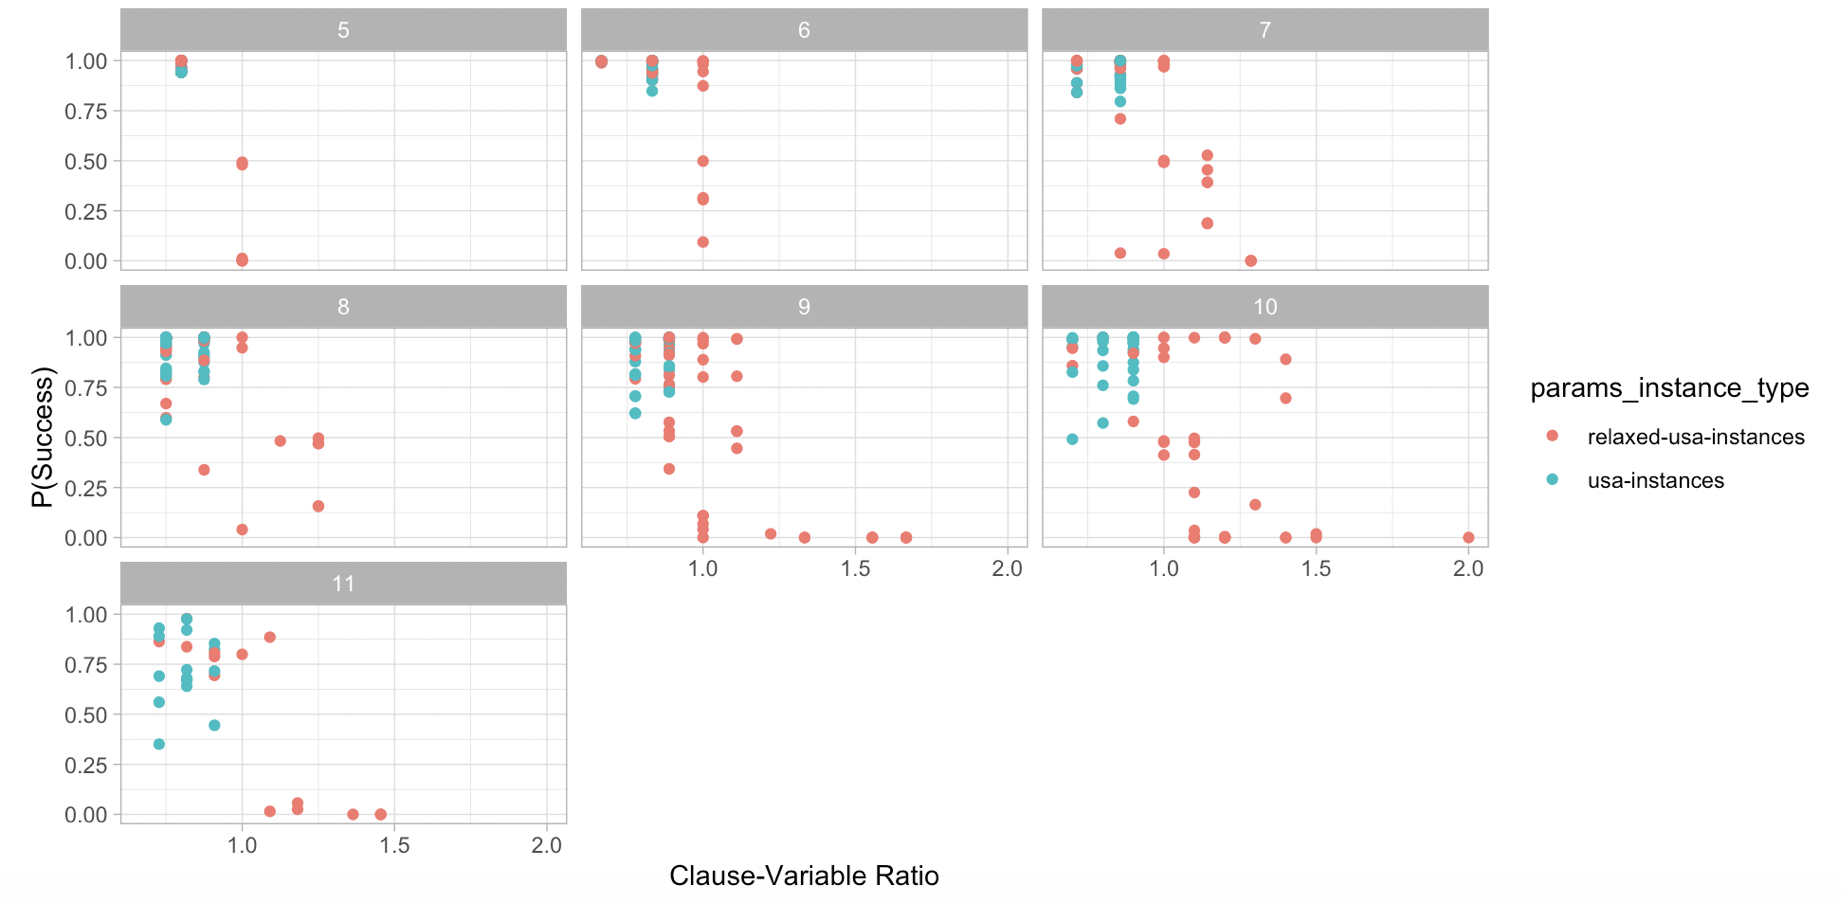
\includegraphics[width=1\linewidth]{./p-success-cvr} \end{center}

\hypertarget{research-overview---entropy}{%
\subsection{Research Overview -
Entropy}\label{research-overview---entropy}}

\begin{center}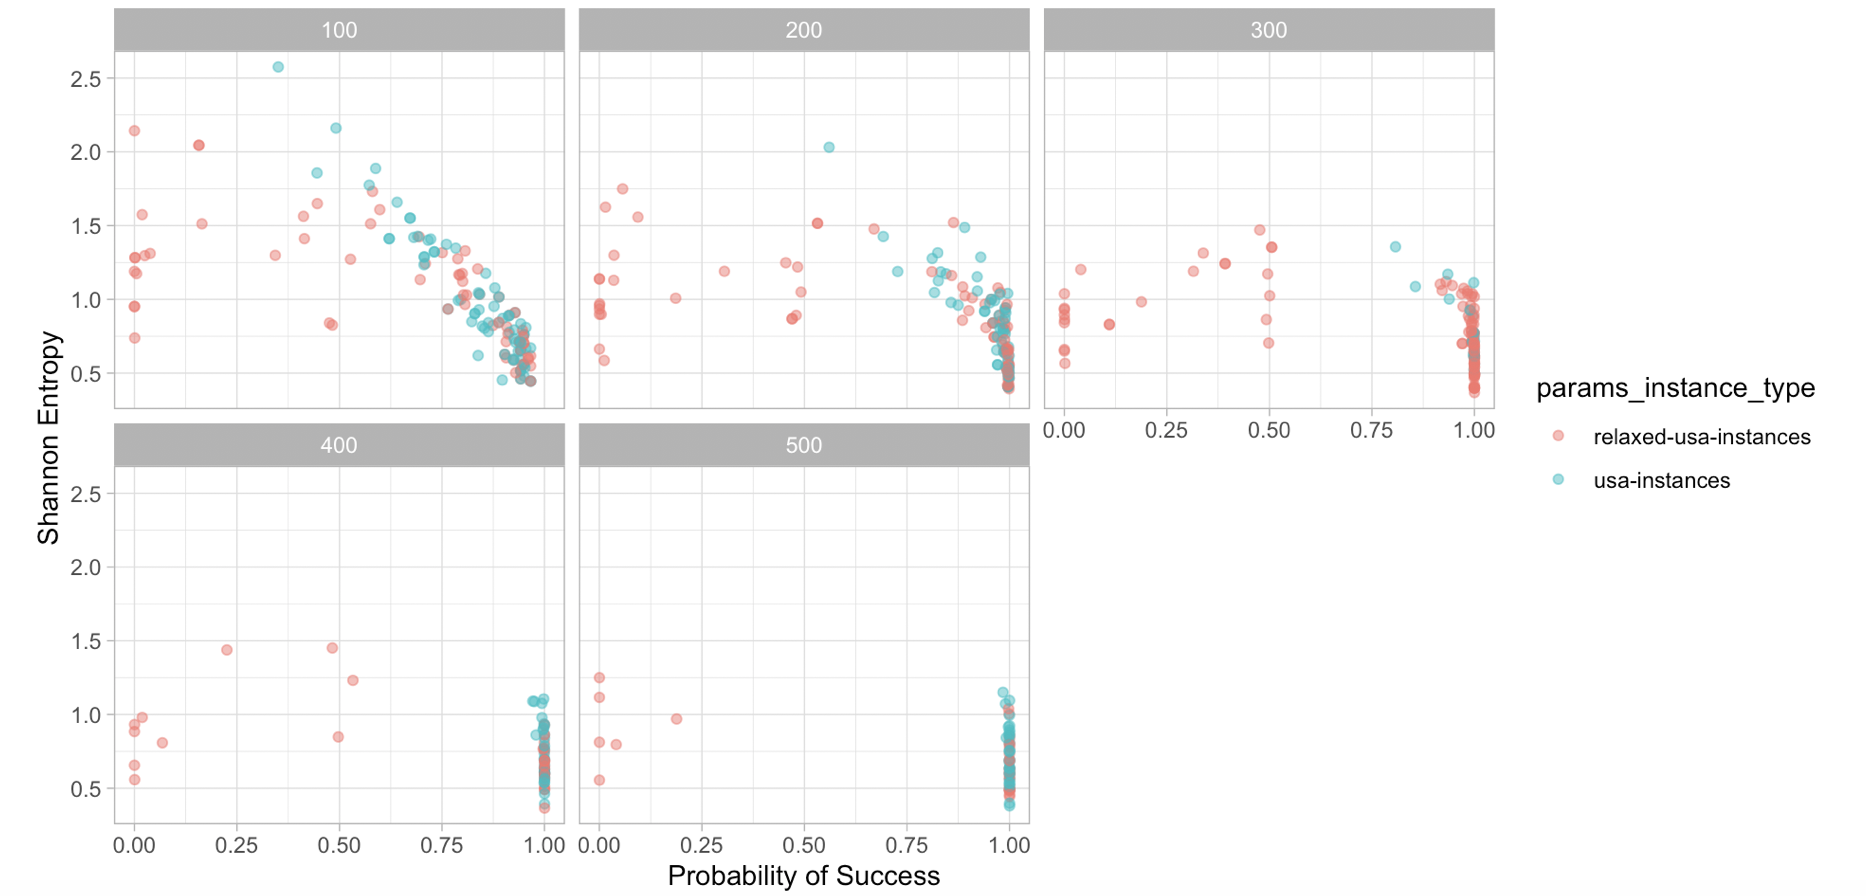
\includegraphics[width=1\linewidth]{./p-success-entropy} \end{center}

\hypertarget{research-overview---minimum-energy-gap}{%
\subsection{Research Overview - Minimum Energy
Gap}\label{research-overview---minimum-energy-gap}}

\begin{center}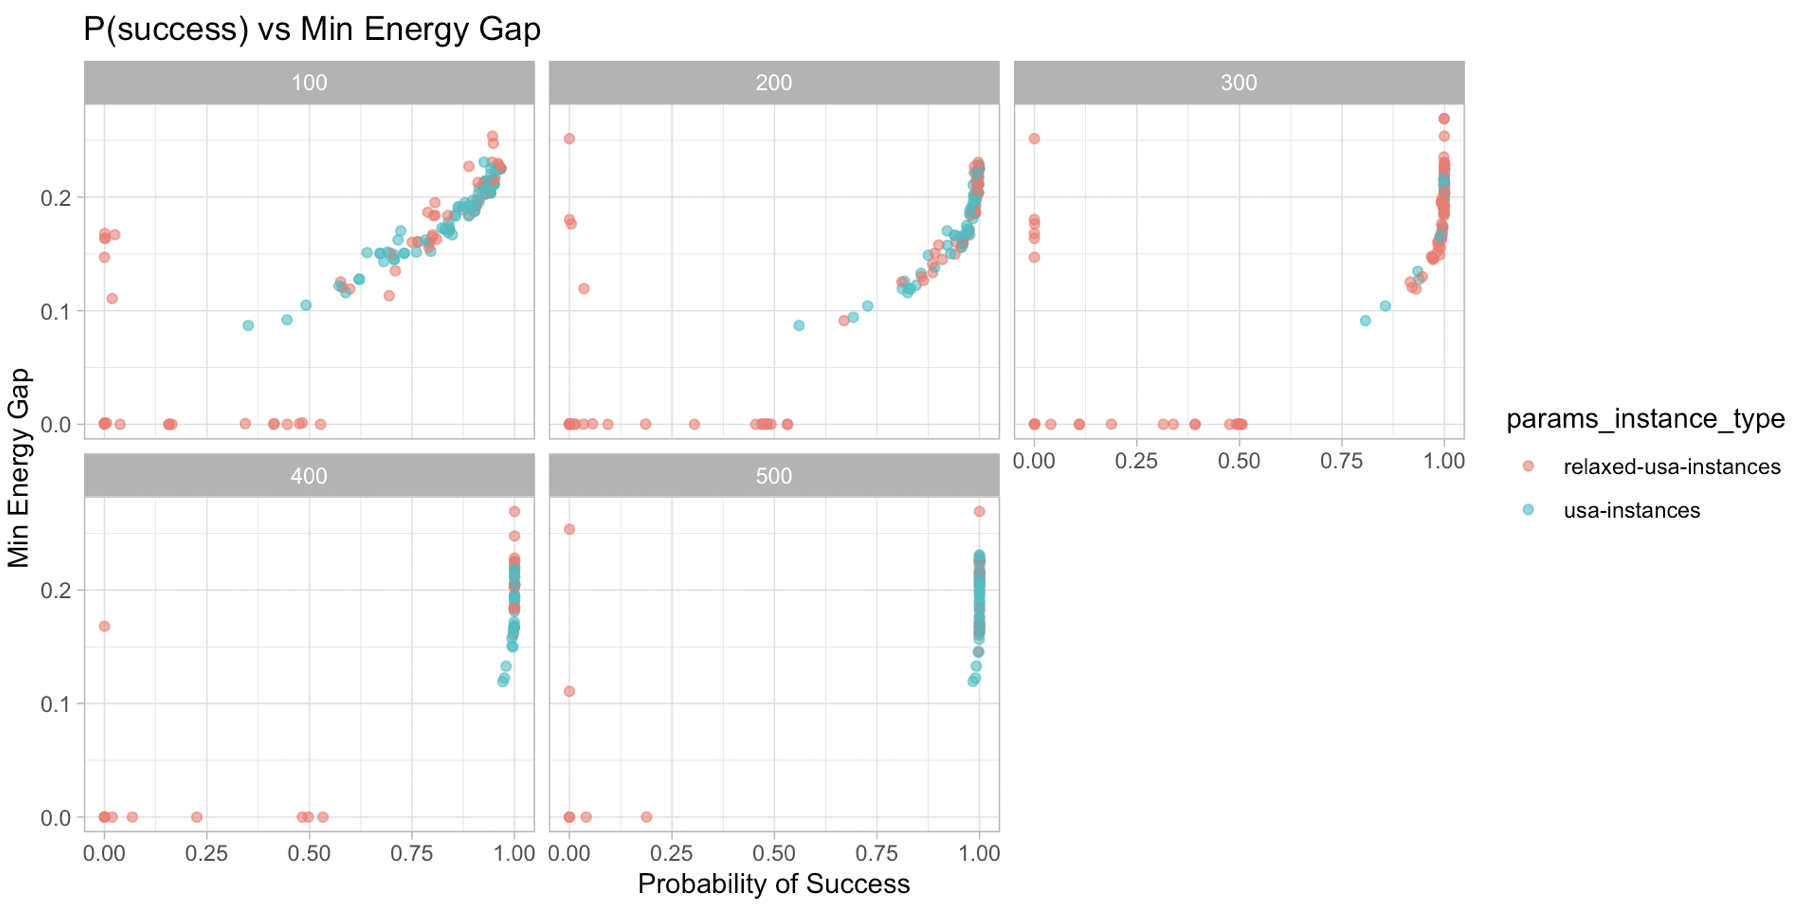
\includegraphics[width=1\linewidth]{./p-success-mgap} \end{center}

\hypertarget{research-overview---results-3}{%
\subsection{Research Overview -
Results}\label{research-overview---results-3}}

\begin{center}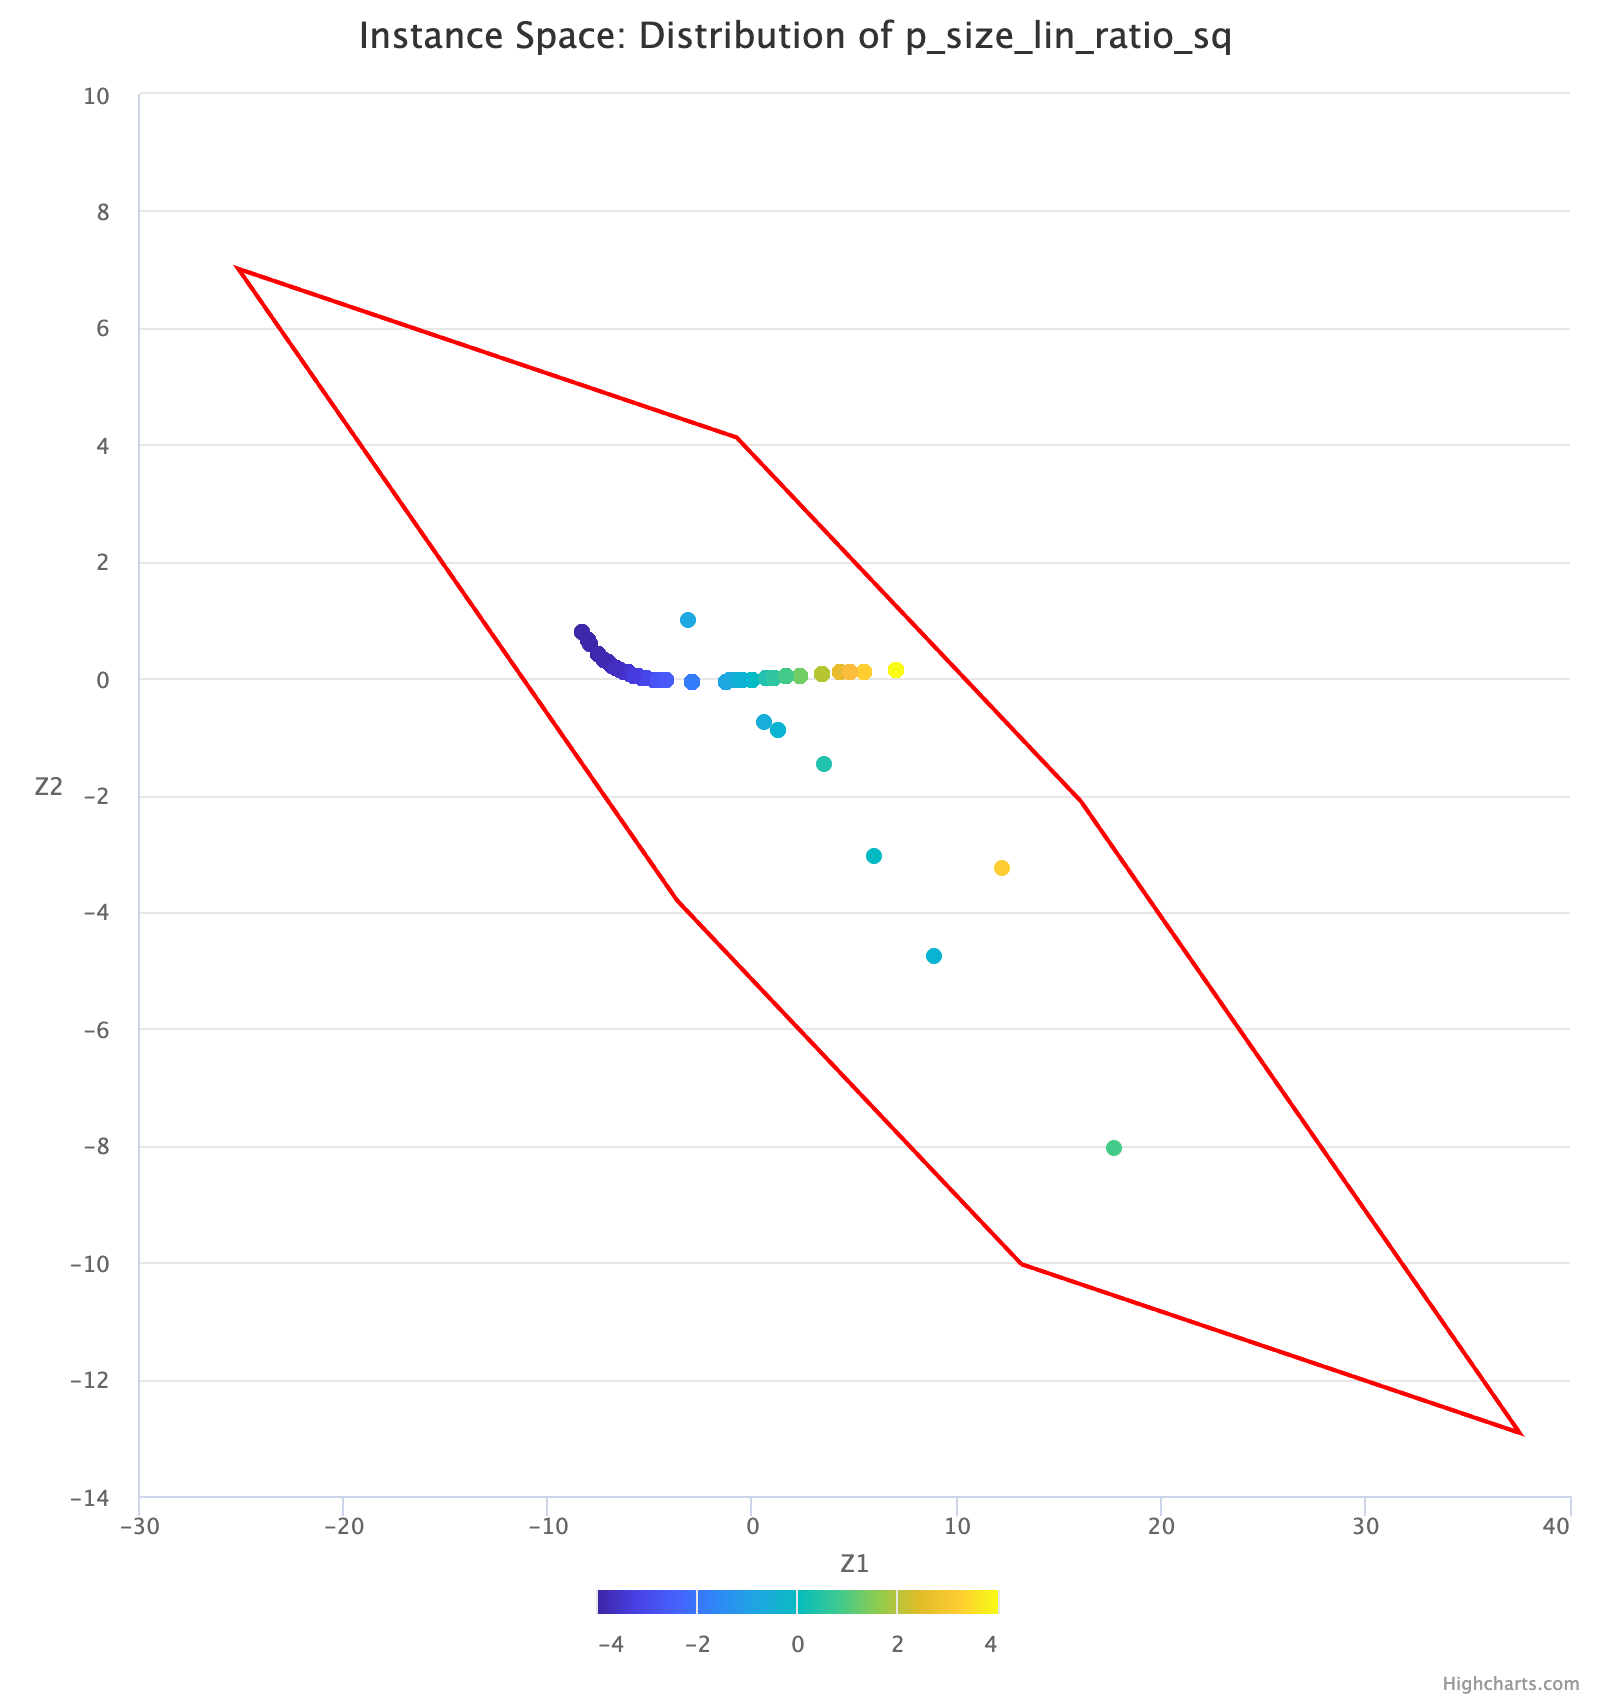
\includegraphics[width=0.5\linewidth]{./matilda-performance-distribution-p-success} \end{center}

\hypertarget{research-overview---results-4}{%
\subsection{Research Overview -
Results}\label{research-overview---results-4}}

\begin{itemize}
\tightlist
\item
  We set a threshold \(\tau=0.95\) for ``good'' or easy instances.
\end{itemize}

\begin{center}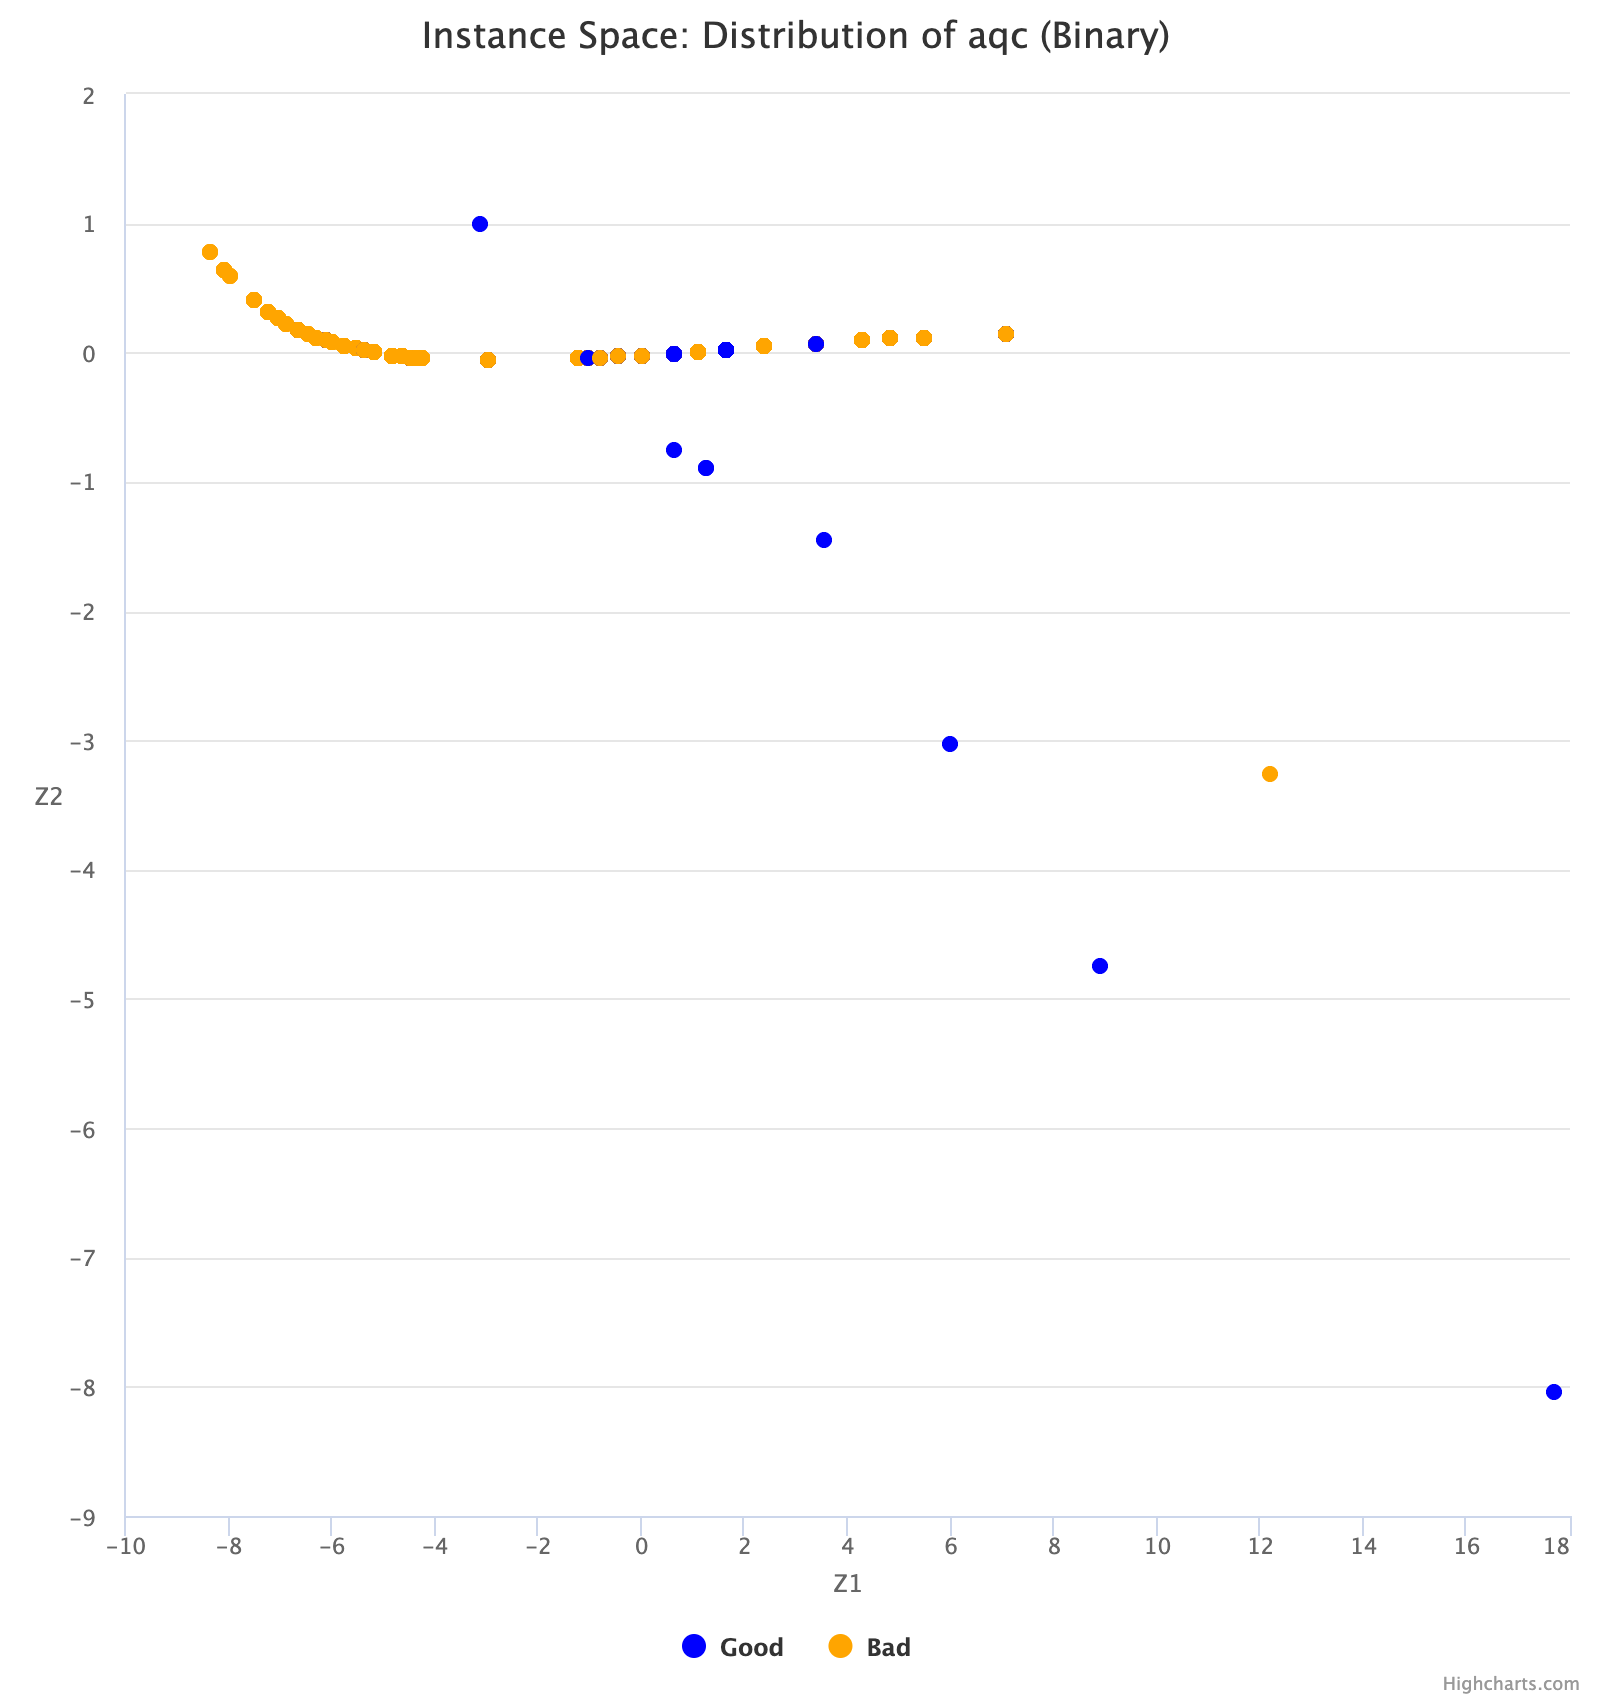
\includegraphics[width=0.5\linewidth]{./matilda-performance-distribution} \end{center}

\hypertarget{next-steps}{%
\section{Next Steps}\label{next-steps}}

\hypertarget{next-steps-1}{%
\subsection{Next Steps}\label{next-steps-1}}

\begin{quote}
\begin{enumerate}
\def\labelenumi{\arabic{enumi}.}
\tightlist
\item
  Generate more instances based on MATILDA results
\item
  Implement more performance metrics on experiments
\item
  Identify which time step \(\Delta t\) is most suitable for evolution
\item
  Investigate the effects of randomising initial Hamiltonians
\end{enumerate}
\end{quote}

\hypertarget{next-steps-2}{%
\subsection{Next Steps}\label{next-steps-2}}

\begin{quote}
\begin{enumerate}
\def\labelenumi{\arabic{enumi}.}
\setcounter{enumi}{4}
\tightlist
\item
  Explore QMC and Matrix-Product States to elicit further insights about
  AQC
\item
  Extend implementation to work on QAOA and VQE with \texttt{QisKit}
\item
  Apply ISA to results from QAOA and run QAOA on Universal Quantum
  Computer
\item
  Extend research to look at other QUBO problems
\end{enumerate}
\end{quote}

\hypertarget{references}{%
\section{References}\label{references}}

\hypertarget{references-1}{%
\subsection{References}\label{references-1}}

\small

\hypertarget{refs}{}
\leavevmode\hypertarget{ref-Born1928}{}%
1. Born M, Fock V (1928) Beweis des adiabatensatzes. \emph{Zeitschrift
für Physik} 51: 165--180.

\leavevmode\hypertarget{ref-Cook1971}{}%
2. Cook SA (1971) The complexity of theorem-proving procedures, In,
\emph{Proceedings of the third annual acm symposium on theory of
computing}, ACM, 151--158.

\leavevmode\hypertarget{ref-Farhi2001}{}%
3. Farhi E, Goldstone J, Gutmann S, et al. (2001) A quantum adiabatic
evolution algorithm applied to random instances of an np-complete
problem. \emph{Science} 292: 472--475.

\leavevmode\hypertarget{ref-Rice1976}{}%
4. Rice JR, others (1976) The algorithm selection problem.
\emph{Advances in computers} 15: 5.

\leavevmode\hypertarget{ref-Smith-Miles2015}{}%
5. Smith-Miles K, Bowly S (2015) Generating new test instances by
evolving in instance space. \emph{Computers \& Operations Research} 63:
102--113.

\leavevmode\hypertarget{ref-Smith-Miles2012}{}%
6. Smith-Miles K, Lopes L (2012) Measuring instance difficulty for
combinatorial optimization problems. \emph{Computers \& Operations
Research} 39: 875--889.

\leavevmode\hypertarget{ref-Smith-Miles2014}{}%
7. Smith-Miles K, Baatar D, Wreford B, et al. (2014) Towards objective
measures of algorithm performance across instance space. \emph{Computers
\& Operations Research} 45: 12--24.

\leavevmode\hypertarget{ref-Hogg2002}{}%
8. Hogg T (2002) Adiabatic quantum computing for random satisfiability
problems. \emph{Phys Rev A 67 022314 (2003)}.

\leavevmode\hypertarget{ref-Young2009}{}%
9. Young AP, Knysh S, Smelyanskiy VN (2009) First order phase transition
in the quantum adiabatic algorithm. \emph{Phys Rev Lett 104, 020502
(2010)}.

\leavevmode\hypertarget{ref-Farhi2009}{}%
10. Farhi E, Goldstone J, Gosset D, et al. (2009) Quantum adiabatic
algorithms, small gaps, and different paths. \emph{arXiv preprint
arXiv:09094766}.

\leavevmode\hypertarget{ref-Latorre2004}{}%
11. Latorre JI, Orús R (2004) Adiabatic quantum computation and quantum
phase transitions. \emph{Physical Review A} 69: 062302.

\leavevmode\hypertarget{ref-Hauke2015}{}%
12. Hauke P, Bonnes L, Heyl M, et al. (2015) Probing entanglement in
adiabatic quantum optimization with trapped ions. \emph{Frontiers in
Physics} 3: 21.

\leavevmode\hypertarget{ref-Lucas2014}{}%
13. Lucas A (2014) Ising formulations of many np problems.
\emph{Frontiers in Physics} 2: 5.

\leavevmode\hypertarget{ref-Mandra2017}{}%
14. Mandrà S, Katzgraber HG (2017) A deceptive step towards quantum
speedup detection. \emph{Quant Sci Technol 3, 04LT01 (2018)}.

\leavevmode\hypertarget{ref-Gabor2019}{}%
15. Gabor T, Zielinski S, Feld S, et al. (2019) Assessing solution
quality of 3SAT on a quantum annealing platform, In, \emph{International
workshop on quantum technology and optimization problems}, Springer,
23--35.

\leavevmode\hypertarget{ref-Li2019}{}%
16. Li RY, Gujja S, Bajaj SR, et al. (2019) Unconventional machine
learning of genome-wide human cancer data. \emph{arXiv preprint
arXiv:190906206}.

\leavevmode\hypertarget{ref-Inoue2020}{}%
17. Inoue D, Okada A, Matsumori T, et al. (2020) Traffic signal
optimization on a square lattice using the d-wave quantum annealer.
\emph{arXiv preprint arXiv:200307527}.

\end{document}
